\documentclass[a4paper]{article}

\usepackage[french]{babel}
\usepackage[T1]{fontenc}
\usepackage[utf8]{inputenc}
\usepackage{amsmath}
\usepackage{graphicx}
\usepackage{lmodern}
\usepackage[left=3cm, right=3cm, bottom=4cm, top=4cm]{geometry}
\usepackage{array}
\usepackage{pdfpages}
\usepackage{listings}
\usepackage{algorithm}
\usepackage{algorithmic}
\usepackage{sidecap}
\usepackage{pdflscape}
\usepackage{hyperref}
\usepackage{tipa}
\usepackage{multirow}
\usepackage[gen]{eurosym}
\usepackage{float}
\DeclareUnicodeCharacter{20AC}{\euro{}}

\usepackage{hyperref}
\hypersetup{    
    colorlinks,
    citecolor=black,
    filecolor=black,
    linkcolor=black,
    urlcolor=black
}

\title{Rapport de conception logicielle}

\author
{
    Pierre-Marie {\sc Airiau}\\
    Valentin {\sc Esmieu}\\
    Maud {\sc Leray}\\
    %Hoel {\sc Kervadec}\\
    %Florent {\sc Mallard}\\
    %Corentin {\sc Nicole}
}

\date{\today}

\newcommand{\pagevierge}[0]{\newpage\thispagestyle{empty}\null\newpage}
\newcommand{\glasir}[0]{Glasir}
\newcommand{\ttable}[0]{{\sc Table}}
\newcommand{\ffigure}[0]{{\sc Figure}}

\newcommand{\nomRepart}[1]{\multicolumn{2}{c||}{\textbf{#1}}}
\newcommand{\nomRepartt}[1]{\multicolumn{2}{c|}{\textbf{#1}}}

\begin{document}
    % Ouh c'est sale.
    \hypersetup{pageanchor=false}
    
\includepdf[pages=1]{figure/couv.pdf}
    \hypersetup{pageanchor=true}
    
    \newpage
    \thispagestyle{empty}
    \mbox{}
    
    \newpage
    
    \setcounter{tocdepth}{2}
    \tableofcontents
    \setlength{\parskip}{10pt}
    
    \newpage
    \thispagestyle{empty}
    \mbox{}

    \newpage
    \section{Introduction}
	La sécurisation des systèmes est une problématique majeure de la société moderne. En ce sens, de nombreuses méthodologies ont été développées~\cite{introSecurite,ADTreeKordy} dans le but d'identifier les risques et de les quantifier. C'est avec cet objectif que le concept d'arbres d'attaque et de défense (ADTrees) a vu le jour.

	Lors de la phase de pré-étude, nous avons pu comprendre l’intérêt pratique de la construction des ADTrees. Leur utilisation permet d'identifier de manière précise les différentes attaques possibles contre un système et de les valuer en termes de coût, de probabilité, etc. ADTool~\cite{adtool_paper} (Attack-Defense Tree Tool), un logiciel libre développé pour l'implémentation de ces arbres sur support informatique, a été mis à disposition pour ce projet. Lors de sa prise en main, des limites ont été constatées. En effet, dans un cas concret d'expertise en sécurité, le système doit faire face à une multitude d'attaques possibles et, par conséquent, l'ADTree qui les modélisera sera de très grande taille. Dans ce cas, il est très difficile pour l'expert d'en extraire des informations pertinentes au premier coup d’œil. Or, ADTool ne fournit pas d'outil permettant à l'utilisateur de simplifier l'analyse de l'arbre. 

	L'objectif de ce projet est donc la création d'un logiciel intégrant ADTool et permettant de faciliter le travail d'un expert en sécurité, en lui fournissant des outils pour analyser facilement ses ADTrees. Ce logiciel portera le nom de \glasir{}  (prononcé [\textipa{glaziK}]). Il s'agit du nom d'un arbre aux feuilles d'or dans la mythologie nordique~\cite{vikingCulture}.

	Ce rapport présente les spécifications fonctionnelles de \glasir{}. Tout d'abord, les limites d'ADTool seront abordées, afin de justifier l'intérêt de \glasir{}. Puis nous détaillerons les différentes fonctionnalités destinées à l'analyse des ADTrees. Enfin, quelques améliorations supplémentaires seront également précisées pour offrir un meilleur confort de création et édition d'arbres. Ces spécifications seront faites en prenant en exemple une situation précise : celle d'un expert en sécurité chargé par le Service des Transports en commun de l'Agglomération Rennaise (STAR) de déterminer les failles de leurs systèmes de paiement.

    \newpage
	
    \section{Architecture globale}
    \label{sec:archiGlobale}
    
    Afin de mieux fixer les idées quant aux fonctionnalités de Glasir, voici une présentation rapide de son utilisation et de son interface.
	    
    \subsection{Diagramme de cas d'utilisation}
    \label{sec:casutil}
    
    L'utilisateur-type de notre outil d'analyse serait un expert en sécurité connaissant déjà le formalisme des ADTrees. C'est donc l'acteur qui a été choisi pour le diagramme de cas d'utilisation de la {\sc Figure}~\ref{fig:use_case}, qui représente l'ensemble des actions possibles à partir de Glasir. Afin de mieux comprendre ce diagramme, un petit rappel sur le formalisme UML s'impose. En effet, les deux termes \og étendre \fg{} et \og inclure \fg{} associés aux différentes flèches ont une signification bien particulière (attention au sens des flèches) :

    \begin{itemize}
    \item A -- \og inclure \fg{} --> B signifie que si A est réalisé, B l'est {\bf forcément} ;
    \item B -- \og étendre \fg{} --> A signifie que si A est réalisé, B {\bf peut} l'être.
    \end{itemize}

    \begin{figure}[H]
        \centering
        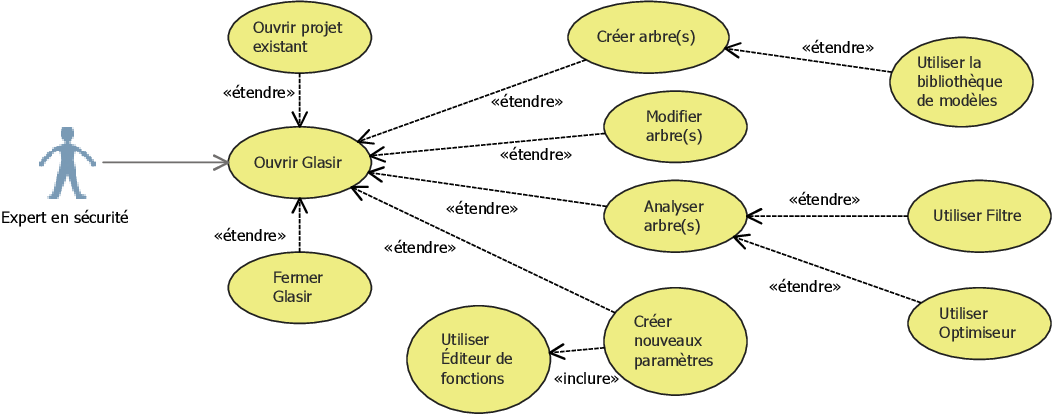
\includegraphics[height=0.5\textwidth]{figure/UseCaseDiagram.png}
        \caption{Diagramme de cas d'utilisation de Glasir.}
        \label{fig:use_case}
    \end{figure}

    Les fonctionnalités de Glasir apparaissent donc maintenant clairement. Grâce à lui, l'utilisateur pourra effectuer les actions suivantes : 

    \begin{itemize}
    \item charger un projet sauvegardé ;
    \item créer de nouveaux ADTrees, en utilisant ou non la bibliothèque de modèles ;
    \item modifier des ADTrees déjà existants ;
    \item analyser les ADTrees du projet en cours, à l'aide du Filtre ou de l'Optimiseur ;
    \item créer de nouveaux paramètres pour ADTool par le biais de l'Éditeur de fonctions.
    \end{itemize}  

    Toutes ces possibilités seront accessibles facilement grâce à une interface utilisateur claire et fonctionnelle, dont un prototype est présenté à la {\sc Section}~\ref{sec:interface}.      
    
    \subsection{Prototype d'interface}
    \label{sec:interface}
    
    La {\sc Figure}~\ref{fig:interface} représente un prototype d'interface pour Glasir. Ce prototype n'est pas définitif, mais permet de donner un avant-goût de l'organisation générale du programme. 

    \begin{figure}[h!]
        \centering
        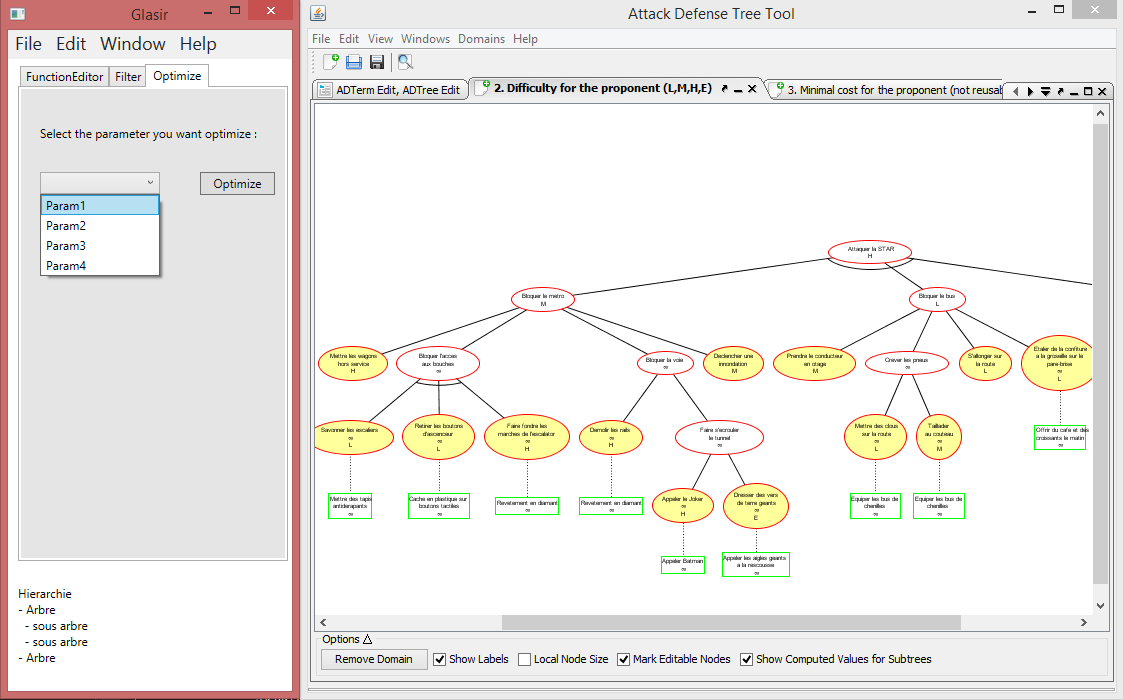
\includegraphics[height=0.72\textwidth]{figure/interface.png}
        \caption{Prototype de l'interface de Glasir.}
        \label{fig:interface}
    \end{figure}
    
    \begin{figure}[h!]
        \centering
        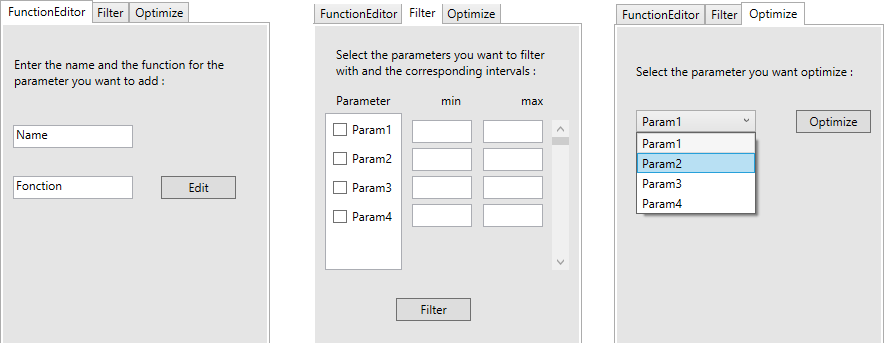
\includegraphics[height=0.42\textwidth]{figure/ongletsGlasir.png}
        \caption{Prototype des panneaux permettant d'utiliser les fonctionnalités de Glasir.}
        \label{fig:panneaux}
    \end{figure}
    
L'interface de Glasir sera scindée en deux parties distinctes : la fenêtre de Glasir à proprement parler (située à gauche sur le prototype de la {\sc Figure}~\ref{fig:interface}), et les fenêtres des instances d'ADTool (situées à droite). Au sein de la fenêtre de Glasir, les fonctionnalités du Filtre, de l'Optimiseur et de l'Éditeur de fonctions seront accessibles facilement. La barre de menu (située en haut à gauche sur le prototype de la {\sc Figure}~\ref{fig:interface}) permettra de créer un nouveau projet, d'en charger un déjà existant, ou encore de sauvegarder le projet courant.
    
    La {\sc Figure}~\ref{fig:panneaux} illustre également un prototype des panneaux qui permettront d'accéder aux fonctionnalités principales de Glasir. Ces fonctionnalités sont détaillées dans les {\sc Sections}~\ref{sec:diagClass} et \ref{sec:modules}.    
    
	\section{Diagramme de classes}
    \label{sec:diagClass}
    
    Le diagramme de classes détaillé dans cette section permet de mieux comprendre l'architecture interne de Glasir. Afin de bien saisir ce diagramme, il est nécessaire de rappeler qu'un ADTree est sauvegardé dans un fichier au format XML.
    
    \subsection{Classe centrale}
    	\label{sec:diagClassCentral}
    	La classe centrale du diagramme est \emph{BigGlasir}, illustrée sur la {\sc Figure}~\ref{fig:bigglasir}. C'est autour d'elle que s'articule l'ensemble des fonctionnalités de Glasir. \emph{BigGlasir} dispose de méthodes permettant de charger un ADTree depuis la bibliothèque de modèles, de lancer des instances d'ADTool afin d'afficher un ADTree, mais également de créer ou de charger un projet. Cette classe possède également des modules, décrit dans la {\sc Section}~{\ref{sec:diagClassMod}}, une bibliothèque de modèles, décrite dans la {\sc Section}~{\ref{sec:diagClassBib}}, et une liste des instances d'ADTool, décrite dans la {\sc section}~{\ref{sec:diagClassADT}}.
    	
    	\begin{figure}[H]
	        \centering
	        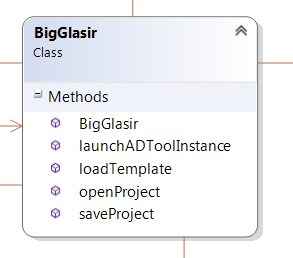
\includegraphics[height=0.3\textwidth]{figure/bigglasir.png}
	        \caption{Classe centrale gérant l'ensemble des autres fonctionnalités.}
	        \label{fig:bigglasir}
	    \end{figure}
    	
    \subsection{Instances d'ADTool}
    	\label{sec:diagClassADT}
    	
    	Comme mentionné dans le rapport de spécification, Glasir gère plusieurs instances d'ADTool pour permettre à l'utilisateur de travailler sur différents ADTrees en même temps\footnote{Pour rappel, ADTool ne peut gérer qu'un seul ADTree à la fois, il n'est par exemple pas possible d'ouvrir deux ADTrees en même temps pour les comparer.}. La classe \emph{ADToolInstance} contient donc le processus d'une instance d'ADTool, ainsi que le fichier de l'ADTree sur lequel l'instance porte. Ce fichier est représenté par la classe \emph{XMLFile}, qui contient un attribut pour représenter le nom du fichier, et des méthodes permettant d'opérer sur ce fichier, comme illustré sur la {\sc Figure}~\ref{fig:instADT}.
    	
    	
    	\begin{figure}[H]
	        \centering
	        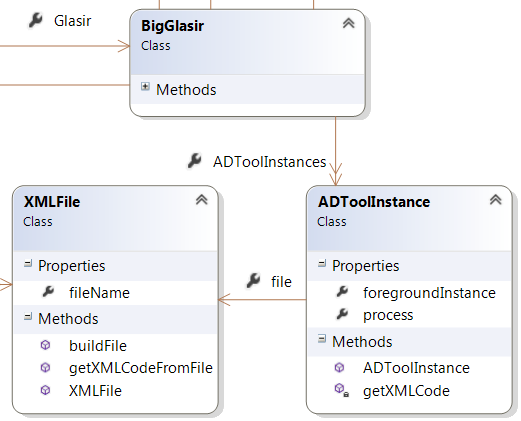
\includegraphics[height=0.5\textwidth]{figure/adtoolinstance.png}
	        \caption{Diagramme de classes des instances d'ADTool.}
	        \label{fig:instADT}
	    \end{figure}
	    


	\subsection{Modules}
    	\label{sec:diagClassMod}    	
    	
    	 Les trois modules principaux de Glasir, c'est-à-dire le Filtre, l'Optimiseur et l'Éditeur de fonction, ont chacun leur propre classe \emph{Filter}, \emph{Optimizer} et \emph{FunctionEditor}. Ces trois classes héritent de \emph{Module}, une classe abstaite contenant les méthodes communes aux trois modules, comme par exemple la méthode permettant d'ouvrir un fichier décrivant un ADTree. De plus, \emph{Module} contient des méthodes abstraites devant être implémentées dans chaque classe héritière, comme la méthode permettant par exemple d'obtenir le fichier résultant d'une opération appliquée par le module. La {\sc Figure}~\ref{fig:mod} illustre l'agencement de ces classes.
    	
    	
    	\begin{figure}[H]
	        \centering
	        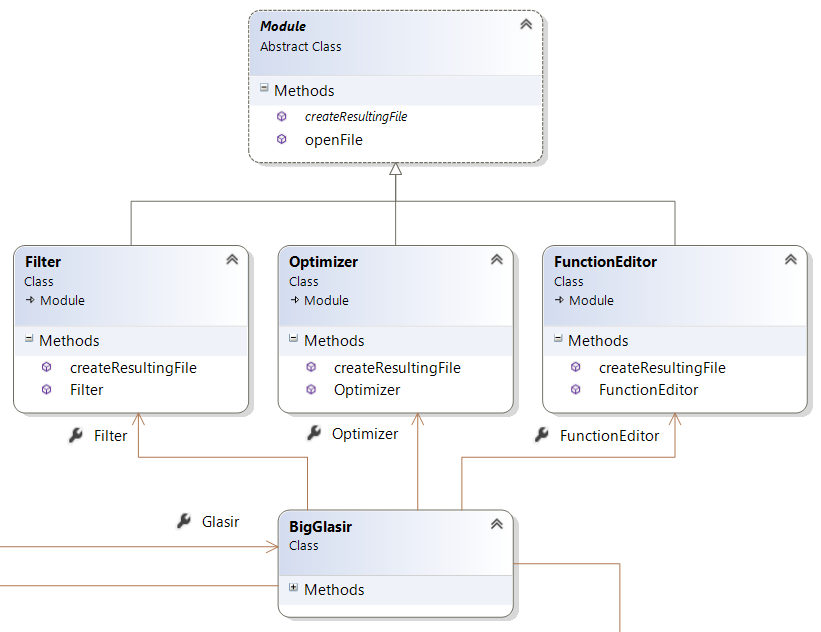
\includegraphics[height=0.7\textwidth]{figure/modules.png}
	        \caption{Diagramme de classes des trois modules de Glasir.}
	        \label{fig:mod}
	    \end{figure}
	    
	    
	\subsection{Bibliothèque de modèles}
    	\label{sec:diagClassBib}
    	La bibliothèque de modèles est constituée de la classe \emph{TemplateLibrary} qui contient une liste des fichiers modèles. Des méthodes permettent d'ajouter ou de supprimer un ADTree de la bibliothèque, ou encore de charger un ADTree dans le projet courant. Les fichiers de cette bibliothèque sont là-aussi représentés par la classe \emph{XMLFile}, comme illustré sur la {\sc Figure}~\ref{fig:lib}.
    	
    	\begin{figure}[H]
	        \centering
	        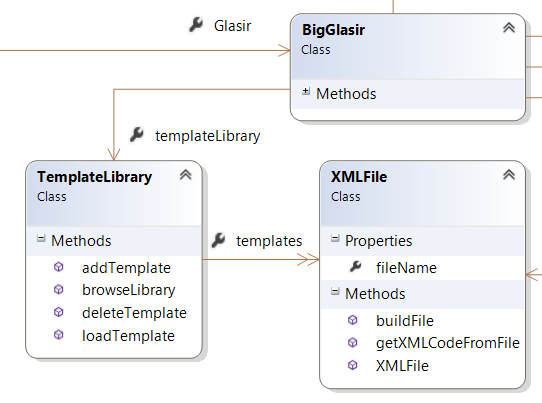
\includegraphics[height=0.5\textwidth]{figure/library.png}
	        \caption{Diagramme de classes de la bibliothèque de modèles.}
	        \label{fig:lib}
	    \end{figure}
	
	\section{Interactions entre modules}
    \label{sec:interactions}
    
    \subsection{Diagramme d'états-transitions}
    	Coucou les loulous
    
    \subsection{Diagramme de séquence}
    	Coucou les loulous
    
    \section{Limites de Glasir}
    \label{sec:limites}

	\section{Organisation}
	\label{sec:orga}
	\subsection{La méthode SCRUM}
		\label{subsec:scrum}

	Afin de définir la méthode de gestion de projet à mettre en place pour la réalisation de \glasir{}, nous avons débattu ensemble des différentes méthodes à notre disposition. A la suite de 	nos discussions en réunions, nous nous sommes dirigés vers une méthode agile proche du \og \textsc{scrum} \fg{}. Ce choix s'est fait sur les points qui sont détaillé ci-dessous :

	L'organisation des rôles que nous avons mise en place depuis le début du projet se base sur un rôle de \og Coordinateur \fg{}, qui est responsable de la réalisation et du rendu d'un livrable (rapport, version logicielle, etc). Ce rôle tourne à chaque nouveau livrable, de sorte que chacun des membres de l'équipe l'exerce au moins une fois. Le rôle de coordinateur que nous avons défini nous a donc semblé correspondre au rôle de ScrumMaster tel que défini dans la méthode \textsc{scrum}.

	Le coordinateur endosse également la responsabilité de Product Owner, qu'il partage avec les encadrants du Projet pour ce qui est de la définition des Objectifs et surtout de l'acceptation des livrables.

	En place de la mêlée quotidienne du \textsc{scrum}, nous nous réunissons une fois par semaine afin de discuter de l'avancement de nos tâches respectives et faire part de nos difficultés. Nous avons décidé d'adopter un rythme hebdomadaire plutôt que quotidien car nous ne travaillerons pas à temps plein sur le projet et ce rythme nous a donc semblé plus adéquat. Nous définissons en fonction des retours en réunion les éventuels ajustements à effectuer la semaine suivante et dans le reste de la planification.

	Enfin, chaque version sera composée de sprints au cours desquels nous nous consacrerons à un sous-ensemble de tâches nécessaires à la réalisation d'une version de \glasir{}. Ces tâches constitueront les Users Stories du projet, et sont détaillées dans la \textsc{sous-section}~\ref{subsec:taches_unitaires}.  
	
	\subsection{Tâches unitaires et estimations}
		\label{subsec:taches_unitaires}

	Nous avons décidé de livrer trois versions de \glasir{} : deux intermédiaires et une finale. Ces dernières ont elles-mêmes été divisées en tâches unitaires, décrites dans cette section.
	
	Pour déterminer le temps nécessaire à l'accomplissement de chaque tâche, nous avons combiné les méthodes d’estimation \og Analogique \fg{} et \og Expertise \fg{}. En effet, la méthode \og Analogique \fg{} consiste à estimer la durée d'une tâche par analogie avec une tâche similaire déjà effectuée (au sein d'un autre projet par exemple). La méthode \og Expertise \fg{}, quant à elle, repose sur le jugement d'un expert. Bien qu'aucun membre de notre groupe ne puisse réellement se considérer comme tel, nos stages respectifs ont tout de même permis d'apporter des avis constructifs sur l'estimation de la durée des tâches.
	
	Les résultats de ces différentes estimations sont décrits ci-après pour chaque version. Il est à noter que les tests et la rédaction de la documentation sont pris en compte dans l'estimation du temps nécessaire à la réalisation de chacune des tâches.
	

		\subsubsection{Version 0.1}
			Huit grandes tâches ont été identifiées pour cette version et sont présentées dans la {\sc Table} \ref{tab:taches_units_1}. 
			\begin{table}[H]
				\centering
				\begin{tabular}{|c|r|l|c|r|}
					\hline
					\textbf{Cible} & \textbf{Id} & \textbf{Tâche} & \textbf{Technologies} & \textbf{Durée}\\
					\hline

					\multirow{5}{*}{\glasir{}} & 1.1 & Squelette interface & WPF & 6h\\
					\cline{2-5}
					 & 1.2 & Gestion fichiers projet & C++ & 20h\\
					\cline{2-5}
					 & 1.3 & Intégration ADTool dans \glasir & JNI & 20h\\
					\cline{2-5}
					 & 1.4 & \'Evaluateur de fonction & Java & 12h\\
					\cline{2-5}
					 & 1.5 & Interface évaluateur & WPF & 8h\\
					\hline

					\multirow{3}{*}{ADTool} & 1.6 & Valuation ADTrees & \multirow{3}{*}{Java} & 18h\\
					\cline{2-3} \cline{5-5}
					 & 1.7 & Refonte langage des ADTrees & & 16h\\
					\cline{2-3} \cline{5-5}
					 & 1.8 & Vue globale des paramètres & & 12h\\
					\hline

					\multicolumn{4}{|l|}{\bf Total} & {\bf 112h}\\
					\hline
				\end{tabular}
				\caption{Tâches associées à la version 0.1.}
				\label{tab:taches_units_1}
			\end{table}
			
			
			La réalisation de cette version sera découpée en trois sprints, présentés ci-dessous :

			\noindent\textbf{Sprint 1} Création de l'interface utilisateur de base de \glasir{}, intégration du logiciel ADTool en tant que fenêtre de \glasir{}, possibilité de création d'un nouveau projet et sa sauvegarde, affichage des différents arbres d'un projet dans un dock sous forme d'arborescence.\newline
			\textbf{Sprint 2} Reconnaissance d'une formule mathématique par le logiciel ADTool, création d'un paramètre en fonction de l'évaluation de cette formule, et l'amélioration de la représentation des arbres sous forme d'une grammaire au sein d'ADTool.\newline
			\textbf{Sprint 3} Affichage de plusieurs paramètres par nœud d'un arbre, possibilité de communication entre le module éditeur de fonction de \glasir{} et la partie création d'un paramètre de synthèse implémentée précédemment dans ADTool.\newline


		\subsubsection{Version 0.2}
			Le développement de la version 0.2 est découpé en cinq tâches, visibles dans la {\sc table} \ref{tab:taches_units_2}.
			\begin{table}[h]
				\centering
				\begin{tabular}{|c|r|l|c|r|}
					\hline
					\textbf{Cible} & \textbf{Id} & \textbf{Tâche} & \textbf{Technologies} & \textbf{Durée}\\
					\hline

					\multirow{4}{*}{\glasir{}} & 2.1 & Algorithme filtrage & C++ & 24h\\
					\cline{2-5}
					 & 2.2 & Interface filtre & WPF & 15h\\
					\cline{2-5}
					 & 2.3 & Multiples instances d'ADTool & C++, WPF & 20h\\
					\cline{2-5}
					 & 2.4 & Affichage arbre filtré & Java, WPF & 16h\\
					\hline

					\multirow{1}{*}{ADTool} & 2.5 & Couper/copier/coller & \multirow{1}{*}{Java} & 25h\\
					\hline

					\multicolumn{4}{|l|}{\bf Total} & {\bf 100h}\\
					\hline
				\end{tabular}
				\caption{Tâches associées à la version 0.2.}
				\label{tab:taches_units_2}
			\end{table}
			
			Nous avons réparti les tâches en trois sprints :

			\noindent\textbf{Sprint 4} Implémentation de l'algorithme de filtrage, permettre l'ouverture de plusieurs instances d'ADTool au sein de différents onglets de l'interface de \glasir{}.\newline 
			\textbf{Sprint 5} Affichage du panneau relatif à ce module au sein de l'interface utilisateur de \glasir{}. Implémentation de la fonction couper/copier-coller.\newline % ou durant le snd sprint?
			\textbf{Sprint 6} Affichage de l'arbre filtré.

		\subsubsection{Version 1.0}
			Quatre tâches ont été identifiées pour la version 1.0 de \glasir{}, regroupées dans la {\sc Table} \ref{tab:taches_units_3}.
			\begin{table}[h]
				\centering
				\begin{tabular}{|c|r|l|c|r|}
					\hline
					\textbf{Cible} & \textbf{Id} & \textbf{Tâche} & \textbf{Technologies} & \textbf{Durée}\\
					\hline

					\multirow{4}{*}{\glasir{}} & 3.1 & Optimiseur & C++, WPF & 30h\\
					\cline{2-5}
					 & 3.2 & Bibliothèque de modèles & C++, WPF & 20h\\
					\cline{2-5}
					 & 3.3 & Harmonisation interface & WPF & 16h\\
					\cline{2-5}
					 & 3.4 & Packaging & ? & 8h\\
					\hline

					\multirow{1}{*}{ADTool} & 3.5 & Ctrl-Z & \multirow{1}{*}{Java} & 16h\\
					\hline

					\multicolumn{4}{|l|}{\bf Total} & {\bf 90h}\\
					\hline
				\end{tabular}
				\caption{Tâches associées à la version 1.0.}
				\label{tab:taches_units_3}
			\end{table}
			
			Les sprints se composeront de :

			\noindent\textbf{Sprint 7} Implémentation de l'algorithme de l'optimiseur, création d'une bibliothèque de modèles.\newline
			\textbf{Sprint 8} Affichage du panneau de l'optimiseur dans \glasir{}, possibilité d'annuler une action dans ADTool.\newline
			\textbf{Sprint 9} Harmonisation de l'interface et réalisation du packaging. \newline

		%TODO estimations
	\subsection{Organisation du groupe et répartition des tâches}
		Lors de la phase de développement de \glasir{}, notre groupe de projet sera réduit à trois étudiants : Pierre-Marie {\sc Airiau}, Valentin {\sc Esmieu} et Maud {\sc Leray}. Les trois autres, Florent {\sc Mallard}, Hoel {\sc Kervadec} ainsi que Corentin {\sc Nicole}, partiront en effet étudier à l'étranger.
		
		Nous comptons donc nous répartir les tâches selon trois composantes générales : Maud L. travaillera principalement sur ADTool, Pierre-Marie A. sur les algorithmes et sur l'interfaçage entre ADTool et \glasir{}, et Valentin E. s'orientera sur l'interface utilisateur de \glasir{}. La {\sc Table} \ref{table:repartition} donne la répartition des tâches plus en détails.
			


		\begin{table}[H]
			\centering
			\begin{tabular}{|l|c|r||c|r||c|r|}
				\hline
				\multirow{2}{*}{} & \nomRepart{Pierre-Marie A.} & \nomRepart{Valentin E.} & \nomRepartt{Maud L.}\\
				\cline{2-7}
				 & {\bf Id tâche} & {\bf Durée} & {\bf Id tâche} & {\bf Durée} & {\bf Id tâche} & {\bf Durée}\\
				\hline
				{\bf Version 0.1} & - & {\bf 38h} & - & {\bf 34h} & - & {\bf 40h}\\
				 & 1.3 & 10h & 1.1 & 6h & 1.2 & 10h\\
				 & 1.4 & 12h & 1.2 & 10h & 1.6 & 18h\\
				 & 1.7 & 16h & 1.3 & 10h & 1.8 & 12h\\
				 & - & - & 1.5 & 8h & - & -\\
				\hline
				{\bf Version 0.2} & - & {\bf 39h} & - & {\bf 33h} & - & {\bf 28h}\\
				 & 2.1 & 24h & 2.3 & 20h & 2.4 & 16h\\
				 & 2.2 & 15h & 2.5 & 13h & 2.5 & 12h\\
				\hline
				{\bf Version 1.0} & - & {\bf 25h} & - & {\bf 23h} & - & {\bf 42h}\\
				 & 3.1 & 15h & 3.1 & 15h & 3.2 & 10h\\
				 & 3.2 & 10h & 3.4 & 8h & 3.3 & 16h\\
				 & - & - & - & - & 3.5 & 16h\\
				\hline
				{\bf Total} & \multicolumn{2}{r||}{{\bf 102h}} & \multicolumn{2}{r||}{{\bf 100h}} & \multicolumn{2}{r|}{{\bf 110h}}\\
				\hline
			\end{tabular}
			\caption{Répartition des tâches, par personne et par version.}
			\label{table:repartition}
			\label{tab:repartition}
		\end{table}


	\subsection{Risques}
		\label{subsec:risques}

	%L'implémentation d'un logiciel comporte toujours des risques. Afin de ne pas nous laisser surprendre par ces derniers, nous avons cherché à lister ceux qui nous venaient à l'esprit.

    % Pour que notre projet se déroule le mieux possible, nous avons listé certains événements susceptibles de nous faire prendre du retard. Ils sont répertoriés dans le tableau\ref{fig:risques}, avec les tâches qu'ils concernent. Nous leur avons ajouté les notions de probabilité (Pr) et de criticité (Cr), sur une échelle de 1 à 3 : 1 pour faible, 2 pour moyenne, 3 pour élevée. Enfin, la dernière colonne cite des solutions possibles pour contre les risques énoncés.

    Dans le but de délivrer ce projet dans les délais, une évaluation des risques a été effectuée. Celle-ci a pour but d'identifier les différents facteurs qui pourraient engendrer des difficultés dans la réalisation des tâches et entraîner ainsi un retard, ou une incapacité à implémenter une partie du cahier des charges. Nous avons associé à chaque élément de cette liste les notions de probabilité (Pr) et de criticité (Cr), sur une échelle de 1 à 3 : 1 pour faible, 2 pour moyenne, 3 pour élevée. Dans le but de réagir au mieux en cas d’apparition de ces aléas, des solutions ont été définies. Le résultat de cette réflexion est présenté dans la \textsc{table}~\ref{fig:risques}. 


	\begin{table}[H]
		\centering
		\begin{tabular}{|p{4cm}|l|l|l|p{4cm}|}
		\hline
            \textbf{Risque} & \textbf{Tâches concernées} & \textbf{Pr.} & \textbf{Cr.} & \textbf{Solution}\\
            \hline
            Mauvaise estimation des durées nécessaires aux tâches unitaires & 
                Toutes & 3 & 3 &
                Bien s'organiser et respecter les délais\\ 
            \hline
            Apparition d'un bug difficile à corriger & 
                Toutes & 3 & 3 &
                Faire des tests unitaires\\
            \hline
            Difficulté à créer une grammaire & 
                1.4 & 1 & 2 &
                Simplifier les expressions à évaluer\\ 
            \hline
            Manque de connaissances techniques & 
                Toutes & 3 & 3 &
                Approfondir nos connaissances\\ 
            \hline
            Rédaction trop tardive de la documentation & 
                Toutes & 2 & 1 &
                Commenter le code au fur et à mesure\\
            \hline
            Mauvaise compréhension du code d'ADTool & 
                Toutes celles sur ADTool & 2 & 2 &
                Contacter le développeur d'ADTool\\ 
            \hline
            Mauvaise communication entre ADTool et \glasir{} & 
                1.4, 2.1, 3.1 & 2 & 3 &
                Utiliser le fichier XML lisible par ADTool\\ 
            \hline
            Perte de temps sur une tâche secondaire & 
                Toutes & 2 & 1 &
                Compter ses heures, faire le point lors des réunions\\ 
            \hline
            Algorithme ralentissant le logiciel & 
                3.1, 2.2 & 1 & 1 &
                Optimiser l’algorithme\\ 
            \hline
            Échec de l'intégration d'ADTool dans \glasir{} & 
                1.2 & 1 & 3 &
                Lancer ADTool séparément\\ 
            \hline
		\end{tabular}
		\caption{Tableau des risques}
		\label{fig:risques}
	\end{table}
	

    \section{Conclusion}

    \bibliographystyle{plain}
    \bibliography{input/biblio}

    % Manoucherie incoming
    \pagevierge
    \ifthenelse{\isodd{\thepage}}
    {\pagevierge}
    {}
    
\includepdf[pages=2]{figure/couv.pdf}
\end{document}
